
\documentclass{beamer}

\usepackage[german]{babel}
\usepackage[utf8]{inputenc}
\usepackage{pdfpages}
\usepackage{graphicx}
\usepackage{amsmath}
\usepackage{amssymb}
\usepackage{amsthm}
\usepackage{mathtools}
\usepackage[font=footnotesize, justification=centering]{caption}
\usepackage{subcaption}


\usetheme{CambridgeUS}
\setbeamertemplate{enumerate items}[default]

%\newtheorem{definition}{Definition}
\newtheorem{thm}{Satz}
%\newtheorem{lemma}{Lemma}

\captionsetup{font=small, justification=centering}
\graphicspath{{../../images/}}
\addto\captionsgerman{\renewcommand{\figurename}{}} % name figures 'Abb.' (change it for babel)

\title[Distanzerhaltende Approximation]{Distanzerhaltende Approximation von Kantenzügen}
\author[N. Klug]{Nikolas Klug}
\institute[Uni Augburg]{Universität Augsburg}
\date{17. Mai 2018}


\begin{document}
	\frame{\titlepage}
	
	\section{Einführung in die Problemstellung}
	\begin{frame}

		\begin{figure}
			\includegraphics<1>[height=0.8\textheight]{maps_zoom1.png}
			\includegraphics<2>[height=0.8\textheight]{maps_zoom2.png}
			\includegraphics<3>[height=0.8\textheight]{maps_zoom3.png}
			\includegraphics<4>[height=0.8\textheight]{maps_zoom4.png}

			\caption{\tiny{Grenze zwischen Deutschland und Österreich. Quelle: \emph{Google Maps}, Stand 8. Mai 2018, \href{https://www.google.de/maps/@47.5869372,11.6674982,9.06z}{https://www.google.de/maps/@47.5869372,11.6674982,9.06z}}}
		\end{figure}
		
	\end{frame}
	
	\begin{frame}{Definition Kantenzug}

		\centering
		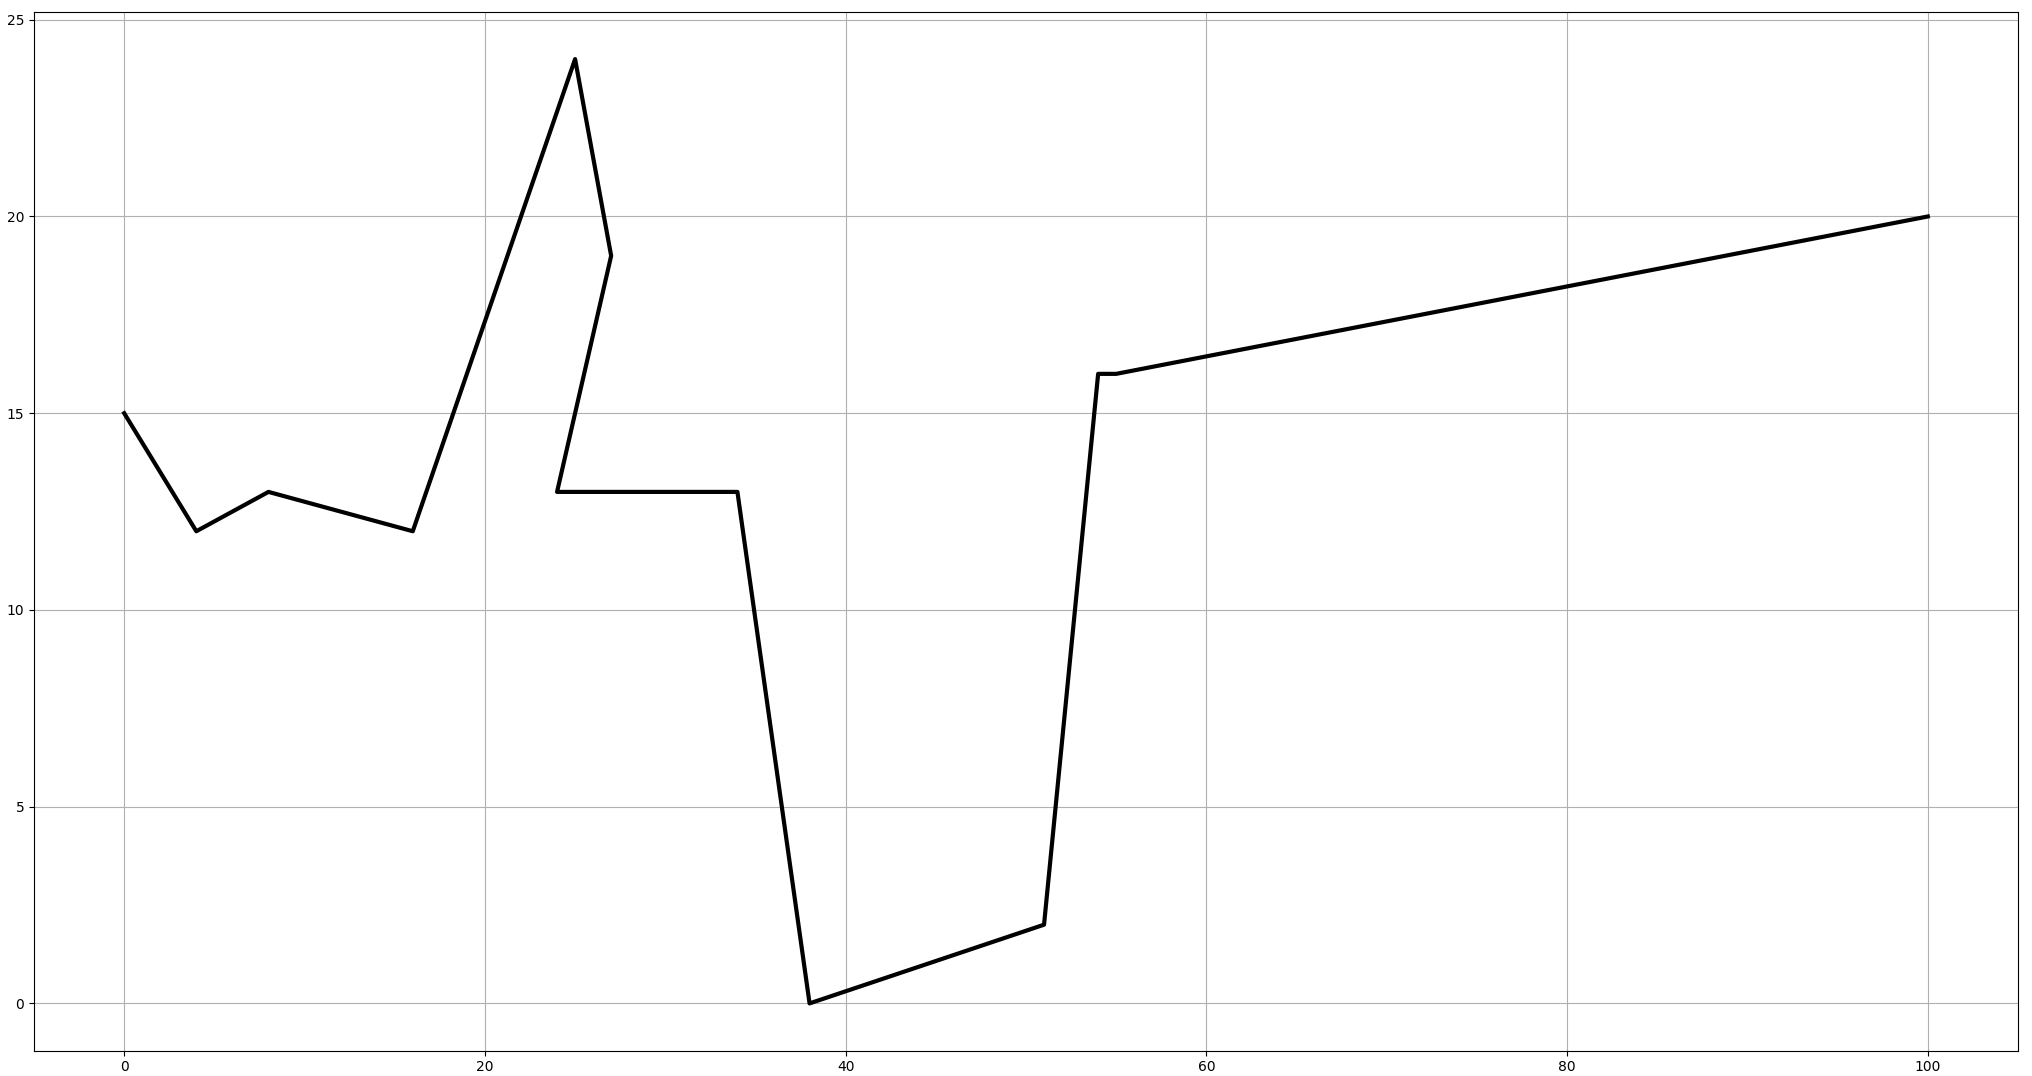
\includegraphics[height=0.6\textheight]{raw_path.png}
		
		\begin{definition}
			Sei $n, d \in \mathbb{N}$ und für $1 \leq i \leq n$ $p_i \in \mathbb{R}^d$.
			Ein \emph{(polygonaler) Kantenzug} $P = (p_1, p_2, \mathellipsis, p_n)$ ist eine Aneinanderreihung von Geradensegmenten, die für $1 \leq i < n$ jeweils die Punkte $p_i$ und $p_{i+1}$ verbinden. 

		\end{definition}
	\end{frame}
	
	\begin{frame}{Definition $t$-distanzerhaltend}
		Sei $P = (p_1, \mathellipsis, p_n)$ ein Kantenzug und $p_i, p_j \in P$.
		\begin{itemize}
			\item<1-> $|p_ip_j|$ ist die euklidische Distanz zwischen $p_i$ und $p_j$.
			\item<2->$\delta(p_i, p_j)~\coloneqq~\sum\limits_{k=i}^{j-1}{|p_kp_{k+1}|}$ ist die Distanz entlang des Pfades.
		\end{itemize}
		\begin{definition}<3->
			Seien $t \in \mathbb{R}$, $t \geq 1$ und $p_i, p_j \in P$. 
			Dann ist die Kante $(p_i, p_j)$ genau dann \emph{$t$-distanzerhaltend}, wenn $\delta(p_i, p_j) \leq t \cdot |p_ip_j|$.
		\end{definition}
		
	\end{frame}
	
	\begin{frame}
		\centering
		$(p_i, p_j)$ \emph{$t$-distanzerhaltend} $\Leftrightarrow$ $\delta(p_i, p_j) \leq t \cdot |p_ip_j|$.
		\vspace{0.5cm}
		\begin{figure}
			\centering
			\begin{subfigure}{.5\textwidth}
				\centering
				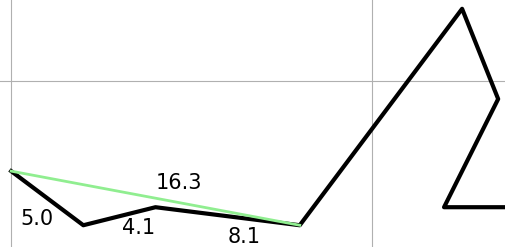
\includegraphics[width=0.95\linewidth]{t_distance_preserving_edge_len.png}
				\caption{$t$-distanzerhaltend}

			\end{subfigure}%
			\begin{subfigure}{.5\textwidth}
				\centering
				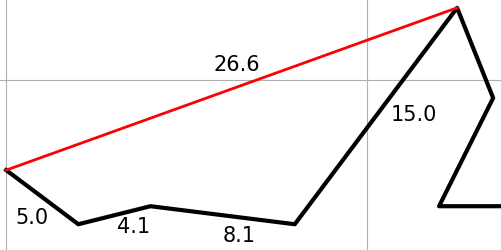
\includegraphics[width=0.95\linewidth]{not_t_distance_preserving_edge_len.png}
				\caption{nicht $t$-distanzerhaltend}
			\end{subfigure}
			\caption{ (nicht) $t$-distanzerhaltende Kanten für $t = 1.2$}
		\end{figure}
	\end{frame}
	
	\begin{frame}{Definition $t$-distanzerhaltende Approximation}
		\begin{definition}
			Ein Kantenzug $Q = (p_{i_1}, p_{i_2}, \mathellipsis, p_{i_k})$ ist genau dann eine \emph{$t$-distanzerhaltende Approximation von $P = (p_1, p_2, \mathellipsis, p_n)$}, wenn beide der folgenden Bedingungen gelten.
			\begin{enumerate}
				\item $\displaystyle 1 = i_1 < i_2 < \mathellipsis < i_k = n$.
				\item $\displaystyle \text{Für alle } 1 \leq l < k \text{ ist die Kante } (p_{i_l}, p_{i_{l+1}})$ des Kantenzugs $t$-distanzerhaltend.
			\end{enumerate}
		\end{definition}
	\begin{figure}
		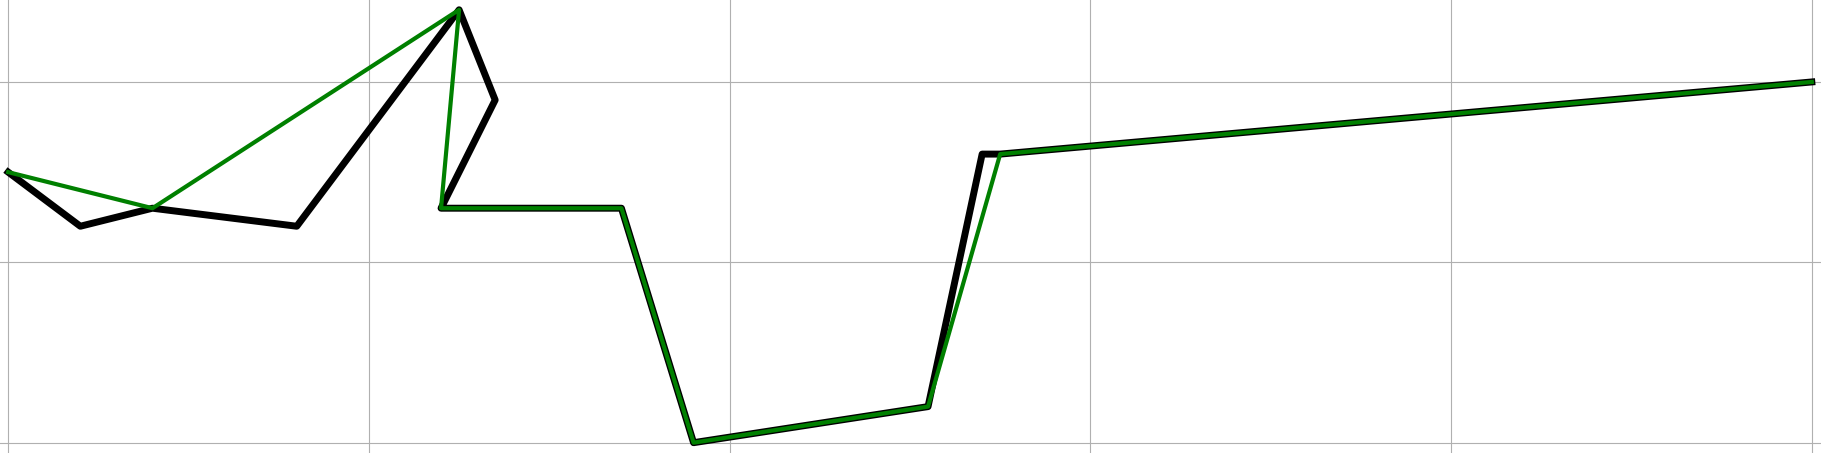
\includegraphics[width=\textwidth]{approximation_example.png}
	\end{figure}
	\end{frame}
	
	\begin{frame}{Problemspezifikation}
		\begin{definition}[Minimum-Vertex-Path-Simplification]
			Liegt ein polygonaler Kantenzug $P$ und eine reelle Zahl $t \geq 1$ vor, soll eine minimale $t$-distanzerhaltende Approximation von $P$ berechnet werden.
		\end{definition}
		\begin{definition}[Minimum-Dilation-Path-Simplification]
			Liegt ein polygonaler Kantenzug $P$ und eine natürliche Zahl $k$ vor, soll der kleinste Wert $t$ bestimmt werden, für den eine $t$-distanzerhaltende Approximation von $P$ mit maximal $k$ Knoten existiert.
		\end{definition}

	\end{frame}
	
	\section{Exakte Algorithmen}
	\subsection{MVPS}
	\begin{frame}{Exakter Algorithmus für das MVPS-Problem}
		Sei $P = (p_1, p_2, \mathellipsis, p_n)$ ein Kantenzug und $t \geq 1$.
		\begin{description}
			\item[Schritt 1:]<1-> Konstruktion des Graphen $G_t = (V, E_t)$, wobei:
			\begin{itemize}
				\setlength{\itemindent}{-1.3cm}
				\item $V = \{p_1, \mathellipsis, p_n\}$
				\item $E_t = \{(p_i, p_j) \in V\times V|\ i < j\ \text{und}\ (p_i,p_j)\ \text{ist $t$-distanzerhaltend}\}$
			\end{itemize}
			\item[Schritt 2:]<3-> Bestimmen eines kürzesten Pfades in $G_t$ von $p_1$ nach $p_n$
		\end{description}
		\uncover<2->{
			\begin{figure}
				\begin{overprint}
					\onslide<2-3>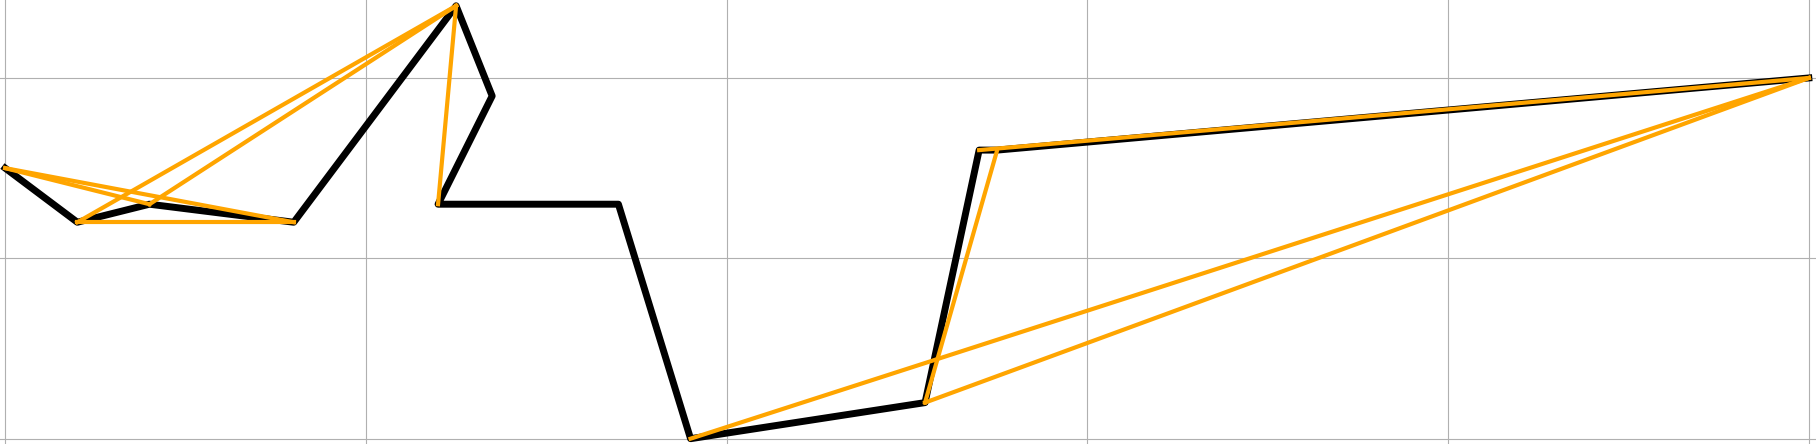
\includegraphics[width=\textwidth]{path_t_distance_preserving_edges_cropped.png}
					\onslide<4->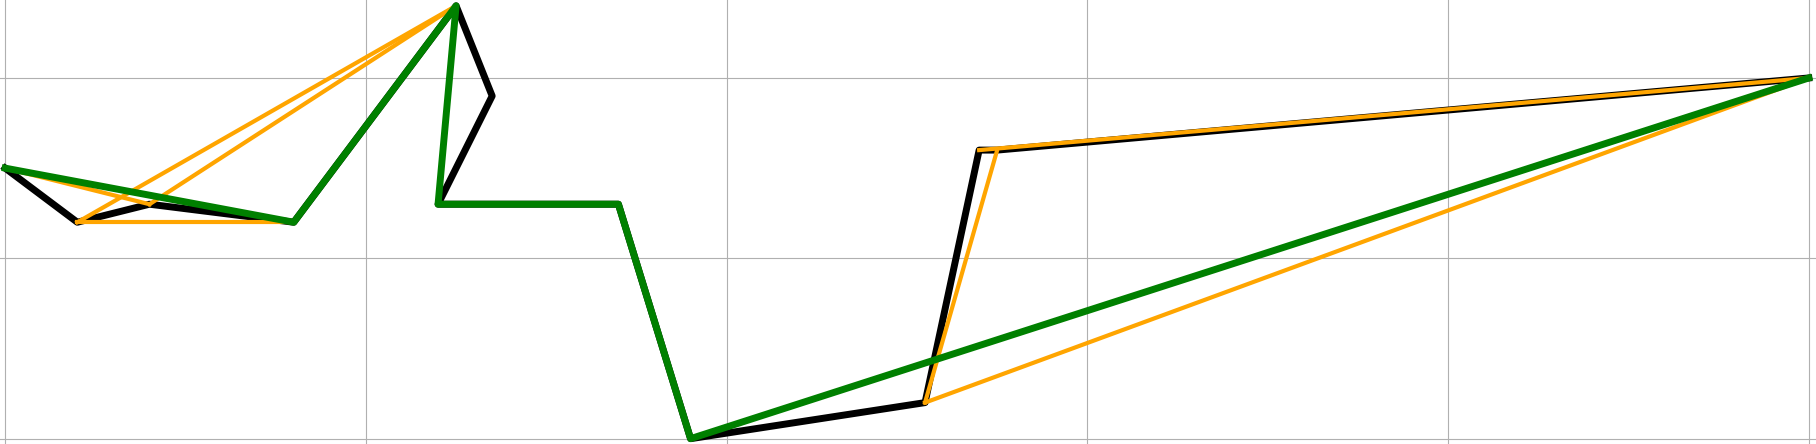
\includegraphics[width=\textwidth]{shortest_path_with_t_edges.png}
				\end{overprint}
				\begin{overprint}
					\onslide<2-3>\caption{$G_t$ für $t = 1.2$}
					\onslide<4->\caption{Kürzester Pfad in $G_t$}
				\end{overprint}
			\end{figure}}
	\end{frame}
	
	\begin{frame}{Laufzeit}
		\begin{columns}
			\begin{column}{0.6\linewidth}
				\begin{description}
					\item[Schritt 1:]<1-> Konstruktion des Graphen $G_t$
					\item[Schritt 2:]<2-> Breitensuche
				\end{description}
			\end{column}
			\begin{column}{0.5\linewidth}
				\begin{description}
					\item[]<1-> $O(n^2)$
					\item[]<2-> $O(n + m) = O(n^2)$
				\end{description}
			\end{column}
		\end{columns}
		\begin{thm}<3->
			Das Minimum-Vertex-Path-Simplification Problem kann für Kantenzüge mit $n$ Knoten in $O(n^2)$ Zeit gelöst werden.
		\end{thm}
	\end{frame}
	
	\begin{frame}{Exakter Algorithmus MVPS}
		Laufzeitbetrachtung und Satz
	\end{frame}
	
	\begin{frame}{Exakter Algorithmus MDPS}
		kurze Wdh MVPS (evtl. grobe Definition)
		
		Lemma: indirekte Proportionalität kappa und t
		
		kurzer Beweis / Beweiserläuterung
		
		evtl. Frage ans Publikum, da einfach
	\end{frame}
	
	\begin{frame}{Exakter Algorithmus MDPS}
		Bildung der Menge aller t-Werte (Größe $O(n^2)$)
		
		Binäre Suche möglich wegen Lemma
		
	\end{frame}
	
	\begin{frame}{Exakter Algorithmus MDPS}
		Laufzeitbetrachtung
		
		+ evtl. Beispielergebnis
	\end{frame}
	
	\begin{frame}{WSPD}
		Definition Well-separated
		
		+ Beispiel Bild
	\end{frame}
	
	\begin{frame}{WSPD}
		Definition WSPD
		
		+ Beispiel Bild (zweidimensional und evtl. mit den Werten aus unserem Beispiel)
	\end{frame}
	
	\begin{frame}{WSPD - Algorithmus}
		Erklärung Split-Tree (binärer Baum)
		
		+ Beispiel mit unseren Werten
	\end{frame}
	
	
	\begin{frame}{WSPD - Algorithmus}
		Satz: Laufzeit
		
		Algorithmus nicht wichtig, nachlesen in Arbeit für Interessierte
		
		Aber wichtig: Die WSPD Mengen werden durch Knoten des Split-Trees repräsentiert, wobei ein Knoten mehrere Mengen repräsentieren kann
	\end{frame}
	
	\begin{frame}{Approximativer Algorithmus WSPD}
		Sei $\epsilon = $..., $s = $ ...
		
		Lemma: 	t-distanzerhaltend $=>$ 1 + e/3 t-distanzerhaltend
				1 + e/3 t-distanzerhaltend $=>$ 1 + e t-distanzerhaltend
				
		+ zweidimensionale Beispiele
	\end{frame}
	
	\begin{frame}{Approximativer Algorithmus WSPD}
		Konstruktion des Graphen H aus "Knoten" der WSPD
		
		Knoten: Elemente der WSPD
		
		Kanten: "?"
	\end{frame}
	
	\begin{frame}{Approximativer Algorithmus WSPD}
		Kanten:
		
		Definition
		
		+ Beispiele
	\end{frame}
	
	\begin{frame}{Approximativer Algorithmus WSPD}
		Satz: Jede Approximation entspricht einem Pfad in H
		
		Beweisskizze
	\end{frame}
	
	\begin{frame}{Approximativer Algorithmus WSPD}
		Satz: Jeder Pfad in H entspricht einer Approximation
	\end{frame}
\end{document}